\section{Auswertung}
\label{sec:Auswertung}

\subsection{Verifizierung des Messverfahrens}
\label{sec:Verifizierung des Messverfahrens}
In \autoref{fig:Geräteeinstellung} ist das Ergebnis des Testscans dargestellt. Daraus wird die doppelte Laufzeit der
Ultraschallwelle zu $\symup{\Delta}\tilde{t}=\qty{8}{\micro\second}$ bestimmt.
Hierfür wurde der zweite Peak (mit gelber Linie markiert) verwendet, da dieser dem einfach reflektierten Puls entspricht.

\begin{figure}[H]
  \centering
  \includegraphics[height=6.5cm]{content/Abbildungen/Geräteeinstellung.pdf}
  \caption{Ausgabe der Vermessung der $\qty{10}{mm}$ Acrylplatte.}
  \label{fig:Geräteeinstellung}
\end{figure}

Mit \eqref{eq:Impuls-Echo} wird somit die Schallgeschwindigkeit in Acryl zu $c_{\symup{exp}}=\qty{2500}{\metre\per\second}$ berechnet.
Verglichen mit dem theoretische Wert von $c_{\symup{theorie}}=\qty{2730}{\metre\per\second}$ ist zwar eine Abweichung festzustellen,
aber prinzipiell konnte die Schallgeschwindigkeit korrekt nachvollzogen werden.
Die Dicke der Platte lässt sich nun bestimmen, indem die berechnete Schallgeschwindigkeit im Programm eingetragen wird.
Der Tiefenscan in \autoref{fig:Plattendicke} ergibt eine Dicke von ca. $\qty{12}{mm}$ (mit gelber Linie markiert), die mit der tatsächlichen
Dicke unter Berücksichtigung von Ableseungenauigkeiten vereinbar ist.

\begin{figure}[H]
  \centering
  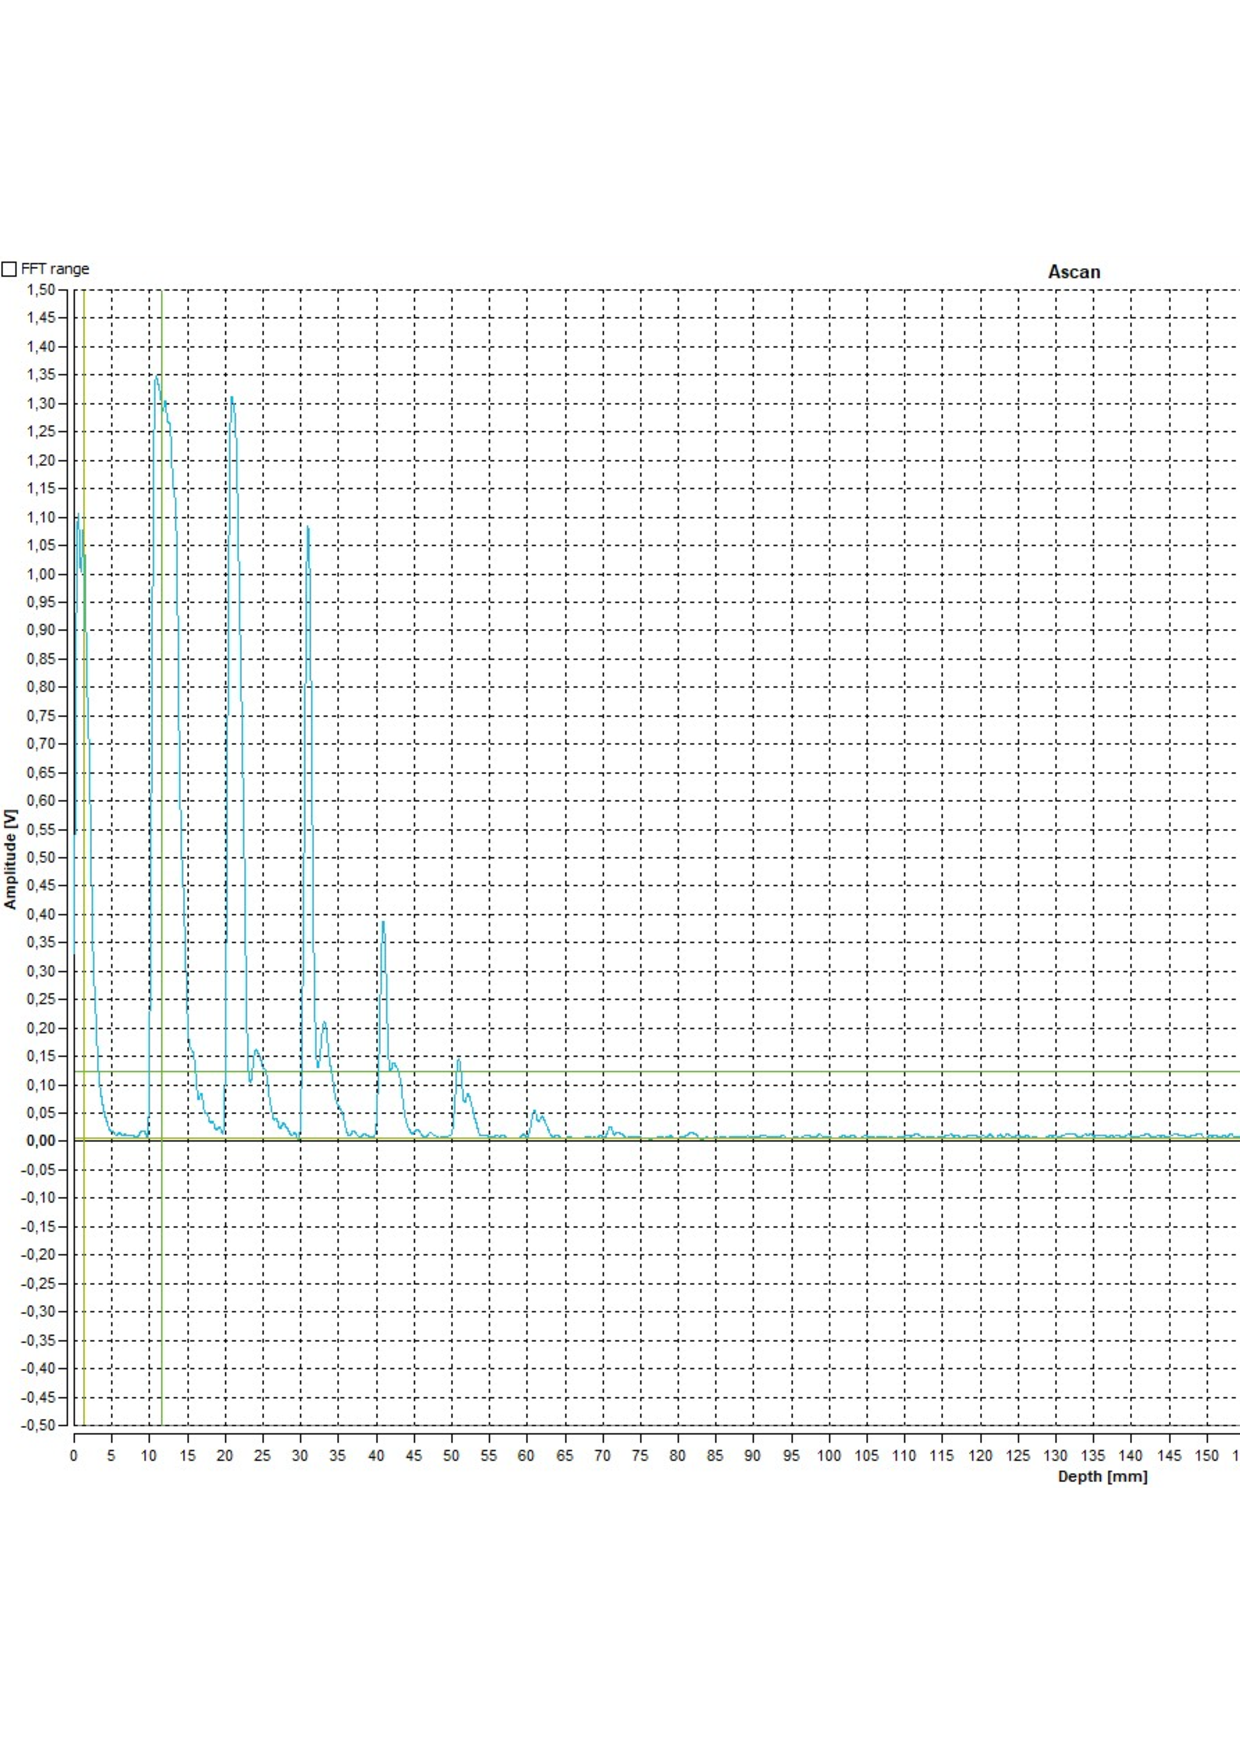
\includegraphics[height=6.5cm]{content/Abbildungen/Plattendicke.pdf}
  \caption{Ausgabe des Tiefenscan der Acrylplatte.}
  \label{fig:Plattendicke}
\end{figure}

Zusammenfassend konnte somit das Verfahren der Ultraschallvermessung als korrekt bestätigt werden,
da sowohl die Schallgeschwindigkeit als auch die Plattendicke mithilfe der Lauftzeit des Ultraschallwelle
berechnet werden konnten.

% $c$-Bestimmung mit Impuls-Echo-Verfahren
\subsection{Messung der Schallgeschwindigkeit mit Impuls-Echo-Verfahren}
\label{sec:c_IE}
Für diesen Teil des Versuches werden Zylinder übereinandergestellt und mit bidestilliertem Wasser gekoppelt, um so mehrere verschiedene Längen 
zu erreichen. Die Laufzeiten der Schallwellen werden abhängig von der Länge der Zylinder in \autoref{tab:c_IE} aufgeführt und in \autoref{fig:c_IE}
graphisch dargestellt.

Nach \eqref{eq:Durchschall} sollte ein linearer Zusammenhang vorliegen. Mithilfe der \textit{python}-Erweiterung \textit{scipy}\cite{scipy} wird eine
lineare Ausgleichsrechnung durchgeführt\footnote{Anm: Der grau hinterlegte Messwert %
wurde nicht bei der linearen Regression betrachtet, da hier sehr wahrscheinlich ein falscher Peak abgelesen wurde.}, welche für die Geradengleichung

\begin{equation*}
  l(\symup{\Delta}t) = m \cdot \symup{\Delta}t + b
\end{equation*}

folgende Parameter liefert:
\begin{align*}
  m_{\symup{IE}} &= \qty{313(21)e-6}{\second\per\metre}\\
  b_{\symup{IE}} &= \qty{0.4(2.1)e-5}{\metre} \\
\end{align*}
Daraus lässt sich schließen, dass die Schallgeschwindigkeit in Acryl hier zu
\begin{equation*}
  c_{\symup{IE}} = \frac{1}{m} = \qty{3.19(0.22)e3}{\metre\per\second}
\end{equation*}
bestimmt wird.
Der Parameter $b$ spiegelt hier die Dicke der Anpassungschicht wider.

\begin{table}[H]
  \centering
  \caption{Daten $c$-Bestimmung mit Impuls-Echo-Verfahren.}
  \label{tab:c_IE}
  \begin{tabular}{S[table-format=3.1] S[table-format=3.0] S[table-format=2.1]}
      \toprule
       {$l\,/\,\unit{\milli\metre}$} & {$\symup{\Delta}\tilde{t}\,/\,\unit{\micro\second}$} & {$\symup{\Delta}t\,/\,\unit{\micro\second}$} \\
      \midrule
         40,4	&  30 & 15,0\\
         61,5	&  46 & 23,0\\
         80,5	&  60 & 30,0\\
        120,5	&  88 & 44,0\\
        101,9	&  75 & 37,5\\
        160,9	& 104 & 52,0\\
        142,0	&  75 & 37,5\\ 
      \bottomrule 
  \end{tabular}
\end{table}

\begin{figure}[H]
  \centering
  \includegraphics{c-Bestimmung_IE.pdf}
  \caption{Graphische Darstellung der Messwertpaare aus \autoref{tab:c_IE} mit Ausgleichsgerade.}
  \label{fig:c_IE}
\end{figure}

% $c$-Bestimmung mit Durchschallungs-Verfahren
\subsection{Messung der Schallgeschwindigkeit mit Durchschallungs-Verfahren}
Die Auswertung der Messwerte erfolt analog zu \ref{sec:c_IE}. Hier liefert die lineare Ausgleichsrechnung die Werte
\begin{align*}
  m_{\symup{D}} &= \qty{361(5)e-6}{\second\per\metre} \\
  b_{\symup{D}} &= \qty{1(5)e-6}{\metre}. \\
\end{align*}
Daraus folgt für die Schallgeschwindigkeit
\begin{equation*}
  c_{\symup{D}} = \qty{2.77(0.04)e+03}{\metre\per\second}.
\end{equation*}

\begin{table}[H]
  \centering
  \caption{Daten $c$-Bestimmung mit Durchschallungs-Verfahren.}
  \label{tab:c_D}
  \begin{tabular}{S[table-format=3.1] S[table-format=2.0]}
      \toprule
       {$l\,/\,\unit{\milli\metre}$} & {$\symup{\Delta}t\,/\,\unit{\micro\second}$} \\
      \midrule
         40,4	& 15\\
         61,5	& 23\\
         80,5	& 30\\
        120,5	& 44\\
      \bottomrule 
  \end{tabular}
\end{table}

\begin{figure}[H]
  \centering
  \includegraphics{c-Bestimmung_D.pdf}
  \caption{Graphische Darstellung der Messwertpaare aus \autoref{tab:c_D} mit Ausgleichsgerade.}
  \label{fig:c_D}
\end{figure}

% Messung der Dämpfung mit Impuls-Echo-Verfahren
\subsection{Messung der Dämpfung mit Impuls-Echo-Verfahren}
Für die Bestimmung des Dämpfungskoeffizienten $\alpha$ wird das Verhältnis der Amplituden der ausgesendeten und der einfallenden Ultraschallwelle
gebildet. Dieses Verhältnis wird logarithmisch gegenüber der doppelten Länge der Acrylzylinder aufgetragen und es wird eine lineare Ausgleichsrechnung 
durchgeführt.\footnote{Anm: Die grau hinterlegten Messwerte wurden für die Ausgleichsrechnung nicht berücksichtigt, da hier davon auszugehen ist, dass 
Kopplung zweier Zylinder nicht ausreichend gut war. Dies hatte vermutlich zur Folge, dass der Peak der eigentlichen Reflexion am Ende des Zylinders
im Hintergrundrauschen untergegangen ist.}
\begin{align*}
  m_{\symup{Dämpfung}} &= \qty{-13.8(1.3)}{\per\metre} \\
  b_{\symup{Dämpfung}} &= \qty{0.9(1.3)}{\metre}
\end{align*}
Nach \eqref{eq:Dämpfung} liegt ein exponenzieller Zusammenhang zwischen Signalstärke und zurückgelegter Strecke vor. Folglich liefert die 
Steigung der linearen Regressiongeraden den Dämpfungskoeffizienten $\alpha$.
\begin{equation}
    \alpha = \qty{13.8(1.3)}{\per\metre}
\end{equation}

\begin{table}[H]
  \centering
  \caption{Daten Dämpfungsbestimmung mit Impuls-Echo-Verfahren.}
  \label{tab:Dämpfung}
  \begin{tabular}{S[table-format=3.1] S[table-format=1.2] S[table-format=1.2]}
      \toprule
       {$l\,/\,\unit{\milli\metre}$} & {$A_{\symup{out}}\,/\,\unit{\volt}$} & {$A_{\symup{in}}\,/\,\unit{\volt}$} \\
      \midrule
         40,4	& 0,84 & 0,63\\
         61,5	& 1,00 & 0,50\\
         80,5	& 1,16 & 0,41\\
        120,5	& 1,22 & 0,11\\
        101,9	& 1,23 & 0,17\\
        160,9	& 1,23 & 0,32\\
        142,0	& 1,23 & 0,30\\ 
      \bottomrule 
  \end{tabular}
\end{table}

\begin{figure}[H]
  \centering
  \includegraphics{Daempfungsbestimmung.pdf}
  \caption{Logarithmische Darstellung des Amplitudenverhältnisses aus \autoref{tab:Dämpfung} mit Ausgleichsgerade.}
  \label{fig:Dämpfung}
\end{figure}

\subsection{Vermessung des Augenmodells}